\documentclass[14pt, a4paper, fleqn, twoside]{extreport}

\usepackage[T2A]{fontenc}
\usepackage[utf8]{inputenc}
\usepackage[english,russian]{babel}
\usepackage{url}
\usepackage{pscyr}

\renewcommand{\rmdefault}{ftm}
\usepackage{setspace}
\onehalfspacing

\usepackage{changepage}
\usepackage{indentfirst} %первый абзац
%%\usepackage{moreverb}
\usepackage[noend]{algorithmic}
\usepackage{amssymb, amsmath, multicol,amsthm}
%%
\usepackage{enumitem, multicol}
\usepackage{titleps,lipsum}
%%
\usepackage{mathrsfs}
\usepackage{verbatim}
\usepackage{pb-diagram}
\usepackage{graphicx}
\graphicspath{ {images/} }
\usepackage{wrapfig}
\usepackage{xcolor}
\definecolor{new}{RGB}{255,184,92}
\definecolor{news}{RGB}{112,112,112}
\usepackage{wallpaper}
\usepackage{float}
\usepackage{hyperref}
\hypersetup{
%colorlinks=true,%
%linkcolor=news,%
linkbordercolor=new,
}



\usepackage{geometry}
\geometry{top=3.5cm,bottom=2cm,left=2cm,right=2cm}

%\flushbottom
%\ruggedbottom

\binoppenalty=5000
\parindent=0pt

\newcommand{\EDS}{\ensuremath{\mathscr{E}}}
\newcommand*{\hm}[1]{#1\nobreak\discretionary{}%
{\hbox{$\mathsurround=0pt #1$}}{}}
\newcommand{\divisible}{\mathop{\raisebox{-2pt}{\vdots}}}
\renewcommand{\theequation}{\arabic{equation}}
\def\hm#1{#1\nobreak\discretionary{}{\hbox{$#1$}}{}}
\newcommand{\bbskip}{\bigskip \bigskip}



%%\DeclareMathOperator{\tg}{tg}
%%\DeclareMathOperator{\ctg}{ctg}

\let\leq\leqslant
\let\geq\geqslant



% Remove brackets from numbering in List of References
\makeatletter
\renewcommand{\@biblabel}[1]{\quad#1.}
\makeatother
% Header and Footer with logo
\usepackage{lastpage,fancyhdr,graphicx}
\usepackage{epstopdf}
\pagestyle{myheadings}
\pagestyle{fancy}
\fancyhf{}
\fancyfootoffset{0in}

\newpagestyle{main}{%
	\setheadrule{.4pt}%
	\sethead
		[\subsectiontitle][][\thepage]
		{\thepage}{}{\sectiontitle} }
\pagestyle{main}
\renewcommand{\headrulewidth}{0pt}  % убрать разделительную линию


\begin{document}

\section*{Численные эксперименты}
\sectionmark{Численные эксперименты}

\subsection*{Одномерное уравнение}
\subsectionmark{Одномерное уравнение}

Рассмотрим следующую задачу для электронной концентрации $n$:

$$\begin{cases}
\dfrac{\partial n}{\partial t} = P-kn+\dfrac{\partial}{\partial z}\left(D\dfrac{\partial n}{\partial z} + u n\right)\\
n|_{z=100\mbox{ }km} = \dfrac{P(z=100\mbox{ }km)}{k(z=100\mbox{ }km)}\\
\left(D\dfrac{\partial n}{\partial z} + u n\right)\bigg|_{z=500\mbox{ }km} = F=const
\end{cases}
$$

Здесь $D$~---~коэффициент амбиполярной диффузии, $u = D\left(\dfrac{1}{T_p}\dfrac{\partial T_p}{\partial z}+\dfrac{m_ig}{2kT_p}\right)$~---~эффективная скорость, $P$ и $kn$~---~слагаемые, отвечающие процессам ионизации при столкновении $O$ и $O+$ и рекомбинации соответственно. В используемой модели температура, концентрация нейтралов, зависимости $D(z), k(z)$ и $P_1(z)$~---~внешние параметры.

Вблизи нижней границы влияние диффузионного слагаемого и переноса пренебрежимо малы по сравнению с процессами фотохимии. Напротив, на верхней части исследуемого высотного интервала преобладают диффузионные процессы, а $P$ и $k$ уже не играют роли. Важной особенностью рассматриваемой задачи является изменение входящих в уравнение коэффициентов $D, P, k, u$ на рассматриваемом отрезке на несколько порядков. Характерные величины на нескольких высотах представлены в следующей таблице: 

\smallskip

\begin{tabular}{|c|c|c|c|}
\hline
&$z_1=200$~км&$z_2=300$~км&$z_3=500$~км\\
\hline
$D$, см$^{2}\cdot$с$^{-1}$&$3{,}1\cdot 10^9$&$3{,}4\cdot 10^{10}$&$4{,}2\cdot 10^{12}$\\
\hline
$k$, с$^{-1}$&$5{,}2\cdot 10^{-3}$&$5{,}5\cdot 10^{-5}$&$1{,}3\cdot 10^{-8}$\\
\hline
$P_1$, см$^{-3}\cdot$с$^{-1}$&$1{,}5\cdot 10^3$&$1{,}2\cdot 10^{2}$&$1{,}3$\\
\hline
$u_\textrm{эфф}/D$, см$^{-1}$&$4{,}8\cdot 10^{-8}$&$4{,}5\cdot 10^{-8}$&$3{,}6\cdot 10^{-8}$\\
\hline
\end{tabular}

\medskip 

Характерные времена различных физических процессов существенно различны, поэтому рассматриваемая задача жесткая. Следовательно, по времени рассматриваем неявные схемы: во всех случаях производную по времени аппроксимируем по формуле $\dfrac{\partial n}{\partial t}\approx \dfrac{n^{j+1}-n^j}{\tau}$, а в правой части все слагаемые берём на следующем временном слое с номером $(j+1)$. С учётом этого замечания далее в записи различных аппроксимаций правой части будем писать только нижние индексы у $n$, подразумевая всегда верхний индекс $(j+1)$.

От разностной схемы требуется выполнение закона сохранения массы, а также сохранение неотрицательности значений $n$ на следующем временном слое, если это свойство было выполнено на предыдущем. Эти требования связаны с отсутствием физического смысла у решений, не сохраняющих массу или содержащих отрицательные значения концентрации.

Перейдем к получению используемых разностных схем. Введём следующие обозначения для шагов по пространству: $$h_i = z_{i+1}-z_i$$ $$h_{i+1/2}=z_{i+1/2}-z_{i-1/2}$$
В точке $z=z_i$ для слагаемого $\dfrac{\partial}{\partial z}D\dfrac{\partial n}{\partial z}$ в разностных схемах используется следующая аппроксимация, полученная двойным применением формулы центральной разности на отрезках $[z_{i-1};z_i]$ и $[z_i; z_{i+1}]$: 
$$\dfrac{\partial}{\partial z}D\dfrac{\partial n}{\partial z} \approx \dfrac{1}{h_{i+1/2}}\left(\dfrac{D_{i+1/2}(n_{i+1}-n_i)}{h_i}-\dfrac{D_{i-1/2}(n_{i}-n_{i-1})}{h_{i-1}}\right)$$
Для слагаемого $\dfrac{\partial}{\partial z}(nu)$ исследуем схемы направленных разностей $\dfrac{u_{i+1}n_{i+1}-u_{i}n_{i}}{h_i}$, а также центральных разностей $\dfrac{u_{i+1}n_{i+1}-u_{i-1}n_{i-1}}{h_{i-1}+h_{i+1}}$.

Нижнее граничное условие (условие Дирихле) аппроксимируется точно, а на верхней границе условие постоянства потока может быть записано несколькими способами. Для данной одномерной задачи используем две различных аппроксимации этого условия:

\begin{itemize}
\item[•] В первом случае поток $\dfrac{\partial n}{\partial z}+\dfrac{u_N}{D_N}\cdot n_N=F$ аппроксимируется с помощью центральных разностей по пространству, что соответствует схеме $$n_N-n_{N-1}+u_N/D_N\cdot h_N\cdot n_N = F\cdot h_N$$
\item[•] Во втором случае для схемы центральных разностей запишем согласованную схему для верхнего граничного случая, получаемую с помощью интегрирования уравнения на $N$-ом шаге по пространству между двумя соседними полуцелыми узлами, а также учёта равенства потока на верхнем полуцелом узле заданной величине $F$: $$h_{N+1/2}\dfrac{n^{j+1}-n^j}{\tau}= F - D_{N-1/2}\dfrac{n_N-n_{N-1}}{h_{N-1}}-\dfrac{1}{2}(u_{N-1}n_{N-1}^{j+1}+u_{N}n_{N}^{j+1})$$
\end{itemize}

Соответственно, в численных экспериментах протестированы три различные разностные схемы: 
\begin{itemize}
\item[•] В схеме $1$ потоковый член и граничное условие аппроксимируются с помощью центральных разностей; 
\item[•] В схеме $2$ только потоковый член в уравнении записывается с помощью центральных разностей, а граничное условие всё еще использует центральные разности;
\item[•] Наконец, схема $3$ имеет согласованные граничное условие и схему, записанные с помощью центральных разностей.
\end{itemize}

Исследуемая задача имеет не зависящее от времени решение, а численные эксперименты показали, что при итерациях по времени происходит установление решения во всех трёх схемах. Используемый шаг по пространству $h = 5$~км и по времени $\tau = 3$~мин обеспечивает сходимость к одной и той же кривой в схемах $1$ и $3$ с характерным временем установления порядка $4-5$ часов (по прошествии этого времени первые несколько значащих цифр в решении уже не изменяются). Схема $2$ также имеет сходимость к стационарному решению, но в отличие от оставшихся двух схем при шаг по пространству $h=5$~км слишком велик, для получения того же самого решения, что и в других двух схемах, необходимо уменьшить шаг хотя бы до $h = 0{,}2$~км.

Результаты расчетов (стационарные решения в зависимости от разного количества узлов по пространству) представлены на следующих графиках (по горизонтальной оси масштаб выбран логарифмическим). Соответственно, $80$, $400$ и $2000$ узлов отвечают шагам по времени $5$~км, $1$~км и $0{,}2$~км.
 
\begin{figure}[H]
\center{
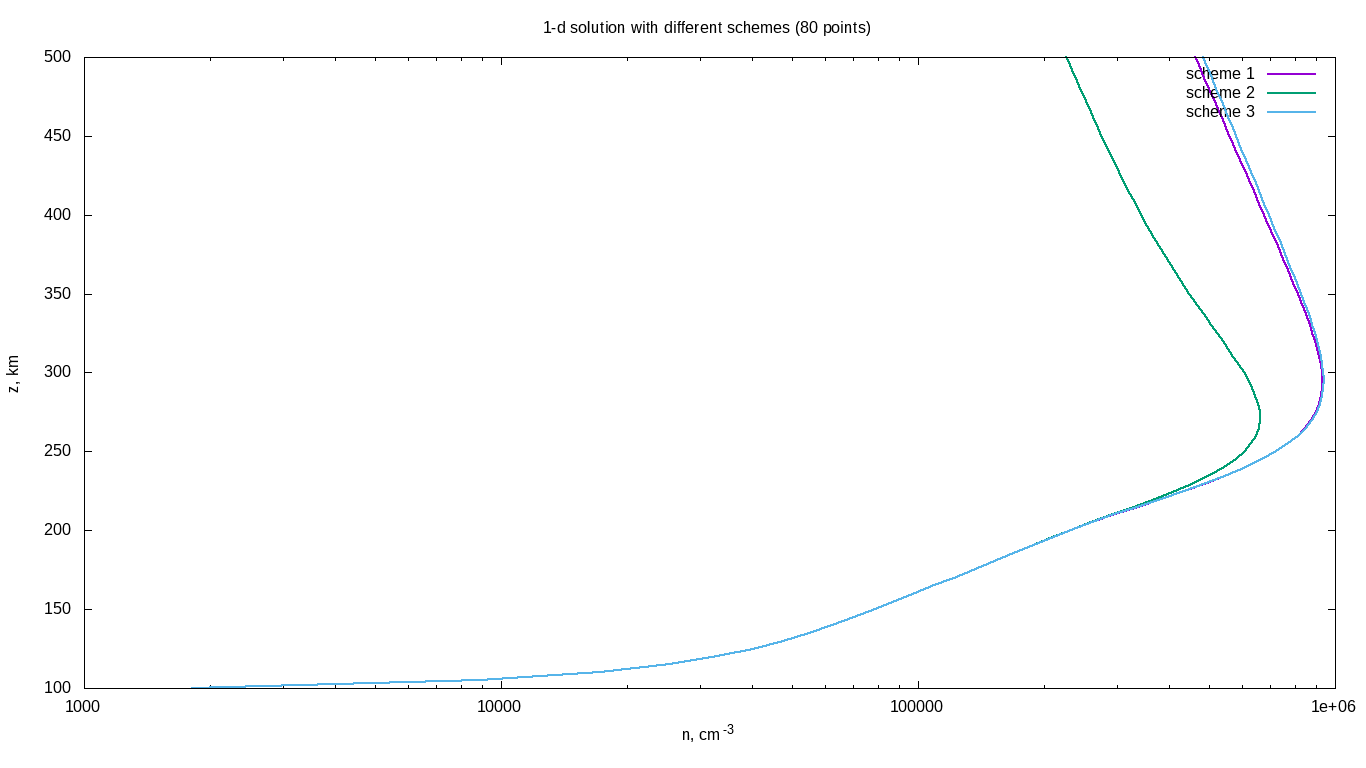
\includegraphics[scale=0.5]{1d_stationary_logscale_80}}
\caption{Стационарные решения на $80$ расчётных узлах.}
\end{figure}

\begin{figure}[H]
\center{
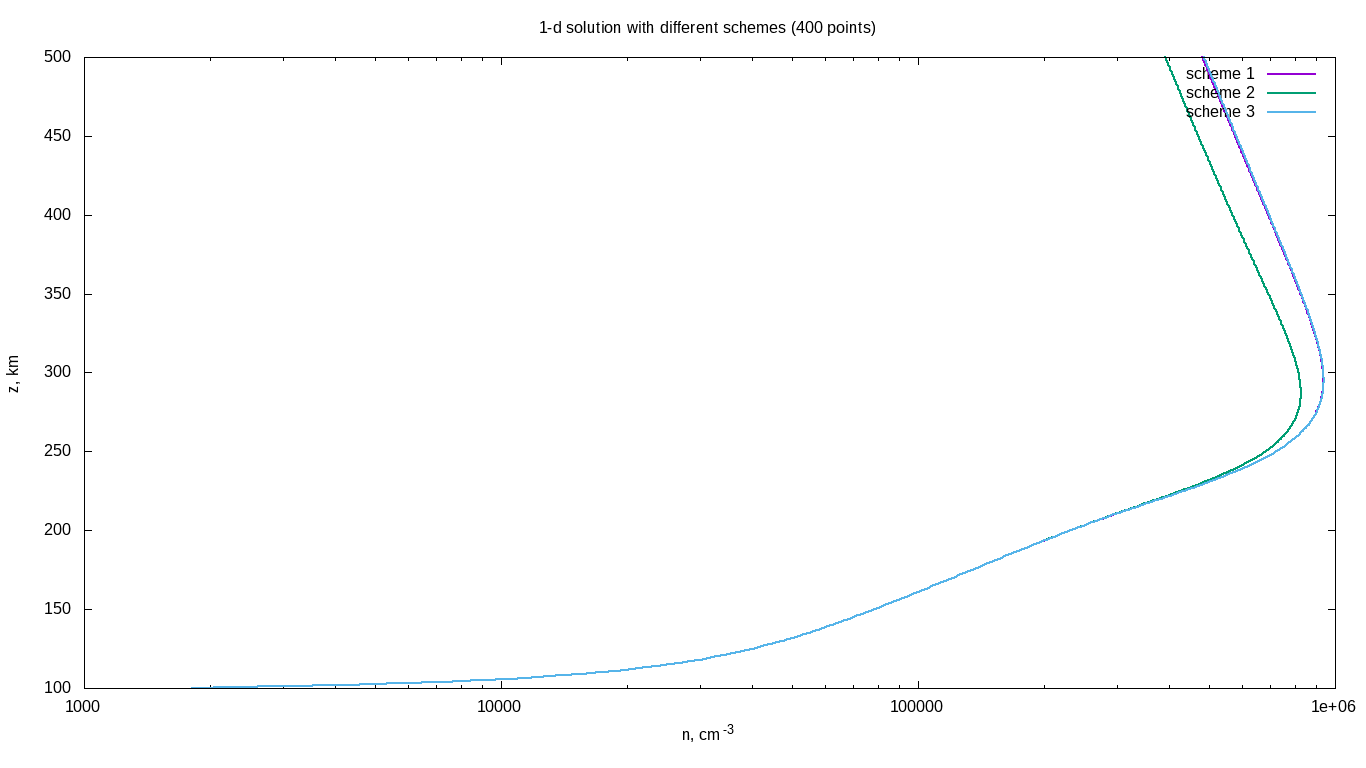
\includegraphics[scale=0.5]{1d_stationary_logscale_400}}
\caption{Стационарные решения на $400$ расчётных узлах.}
\end{figure}

\begin{figure}[H]
\center{
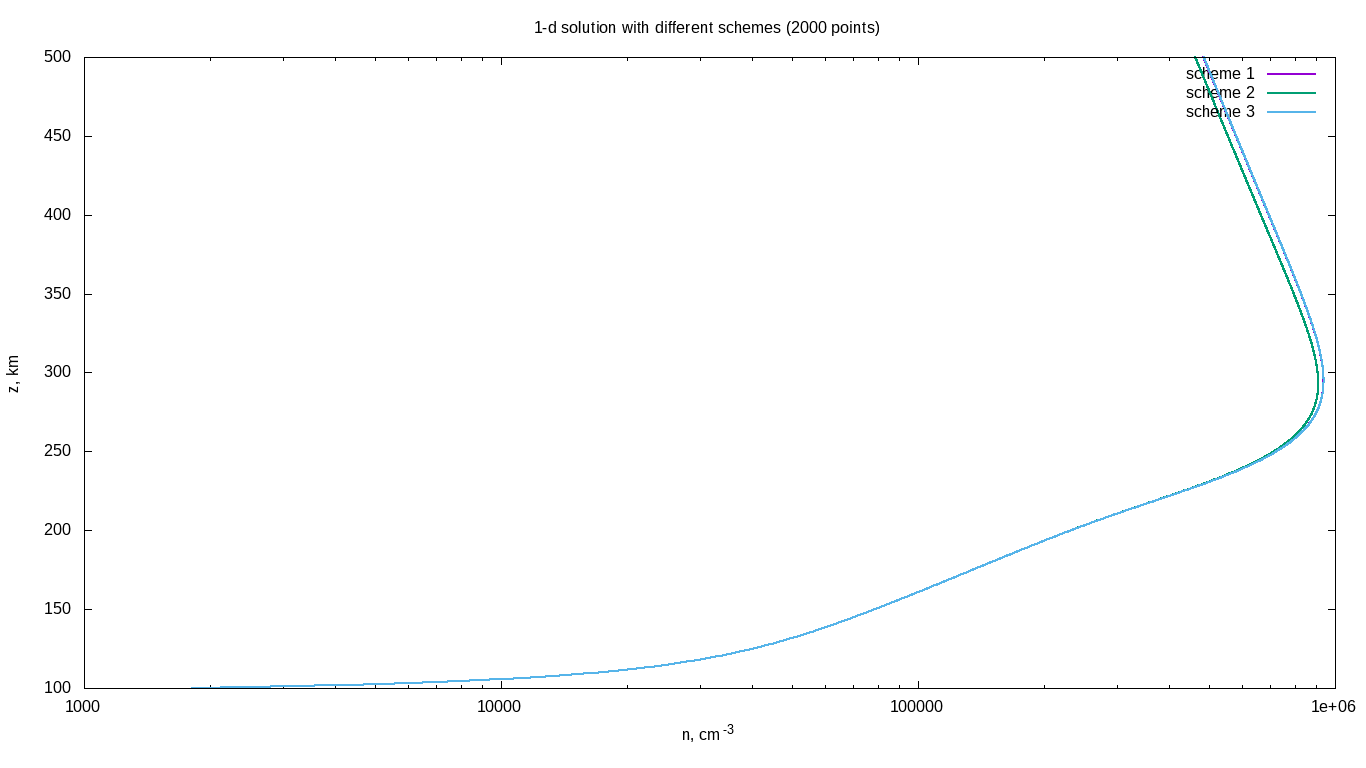
\includegraphics[scale=0.5]{1d_stationary_logscale_2000}}
\caption{Стационарные решения на $2000$ расчётных узлах.}
\end{figure}

Полученное решение позволяет исследовать чувствительность к изменению различных входящих в уравнение внешних параметров: температурам, концентрациям нейтральных молекул, фотоионизации и рекомбинации. На следующих ниже графиках представлены результаты варьирования каждого из параметров в отдельности на $10\%$ и $20\%$ (в обе стороны). В каждом случае вычислено стационарное решение при изменённом параметре, на всех графиках средняя кривая отвечает невозмущенному уравнению.

\medskip

Варьирование входящих в уравнение температур показывает, что наибольшую чувствительность решение имеет к температуре нейтральных молекул. Изменение концентрации нейтральных молекул~---~атомарного кислорода, молекулярного кислорода и азота показывает, что наибольшая чувствительность решения отвечает изменению концентрации атомарного кислорода, а чувствительности к изменению концентраций атомарного кислорода и азота приблизительно одинаковы.

\medskip

\begin{figure}
\center{
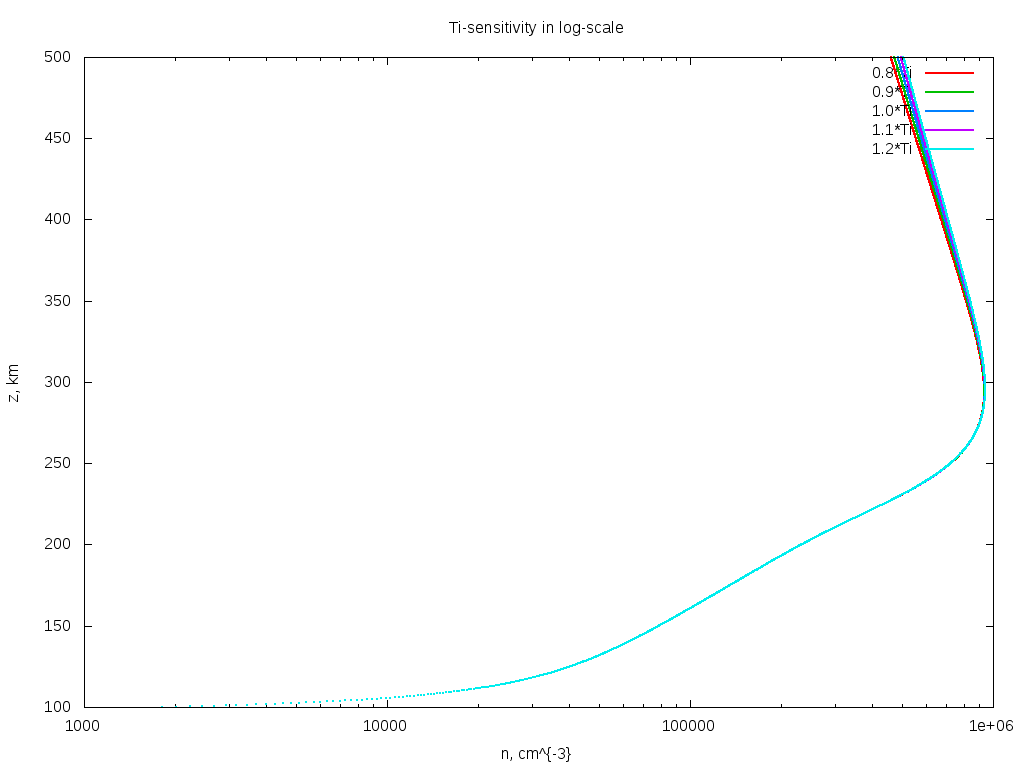
\includegraphics[scale=0.5]{Ti-sensitivity_log}}
\caption{Чувствительность к изменению температуры ионов.}
\end{figure}

\begin{figure}
\center{
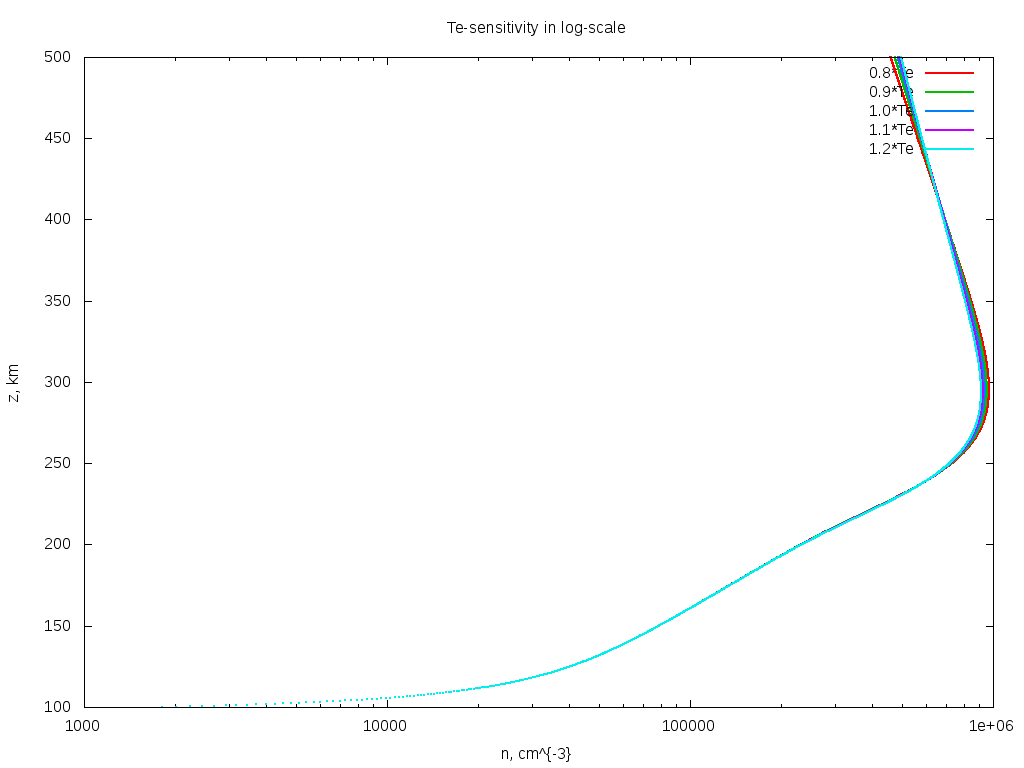
\includegraphics[scale=0.5]{Te-sensitivity_log}}
\caption{Чувствительность к изменению температуры электронов.}
\end{figure}

\begin{figure}
\center{
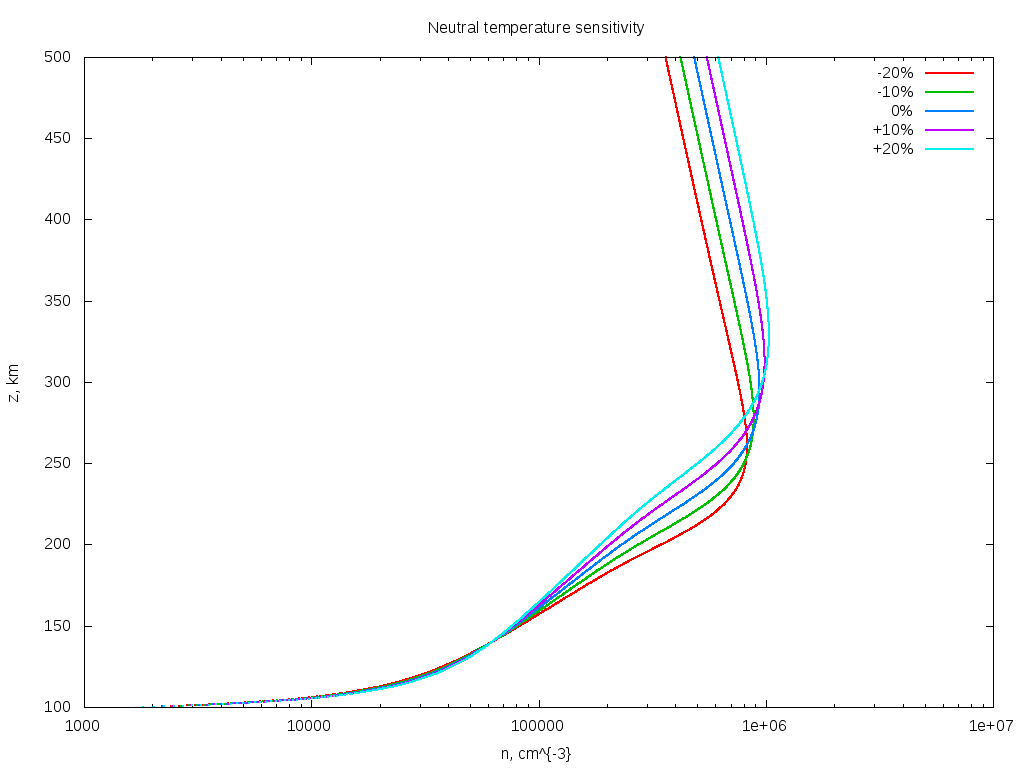
\includegraphics[scale=0.5]{Tn-sensitivity_log}}
\caption{Чувствительность к изменению температуры нейтральных молекул.}
\end{figure}

\begin{figure}
\center{
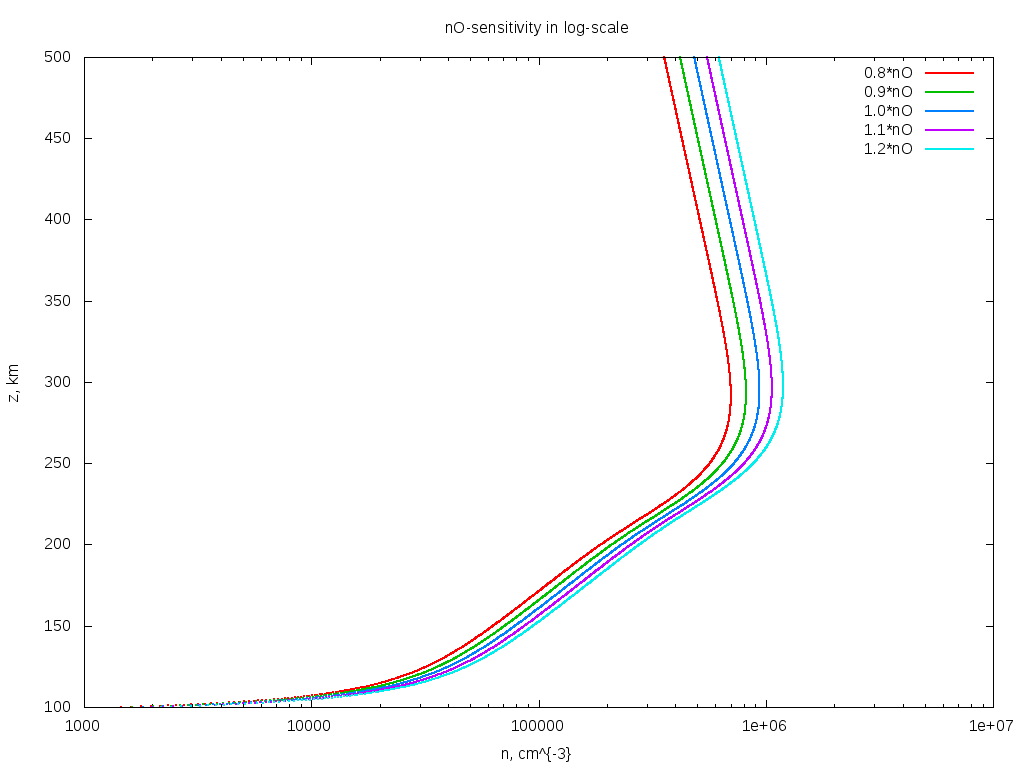
\includegraphics[scale=0.5]{nO-sensitivity_log}}
\caption{Чувствительность к изменению концентрации атомарного кислорода.}
\end{figure}

\begin{figure}
\center{
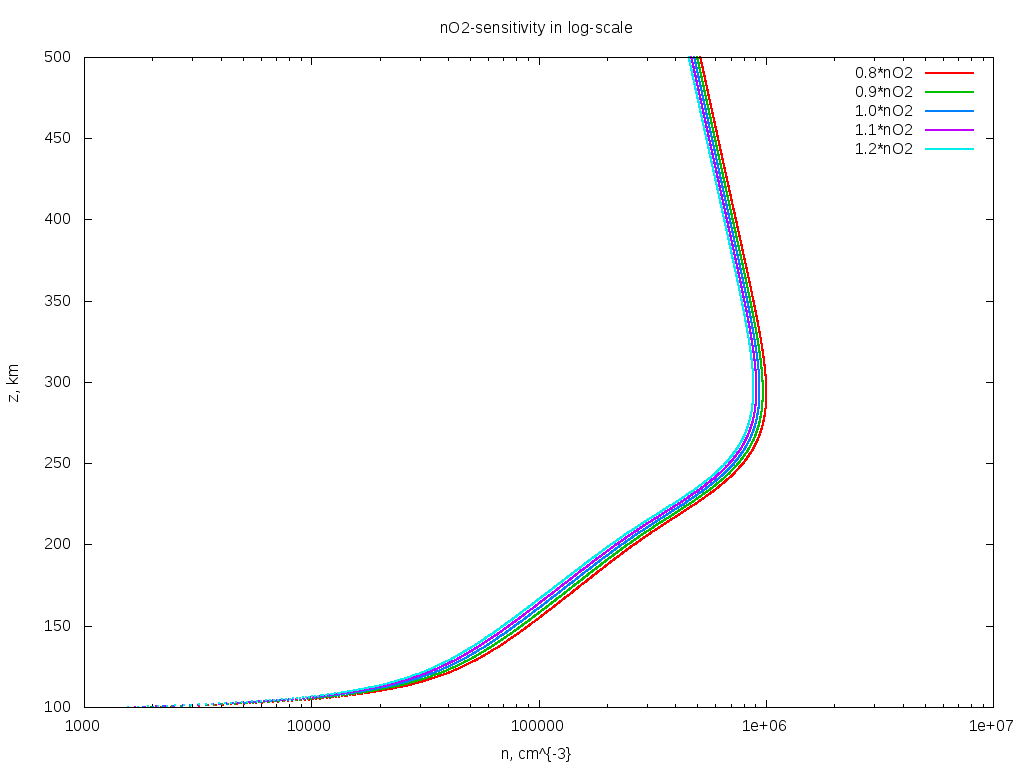
\includegraphics[scale=0.5]{nO2-sensitivity_log}}
\caption{Чувствительность к изменению концентрации молекулярного кислорода.}
\end{figure}

\begin{figure}
\center{
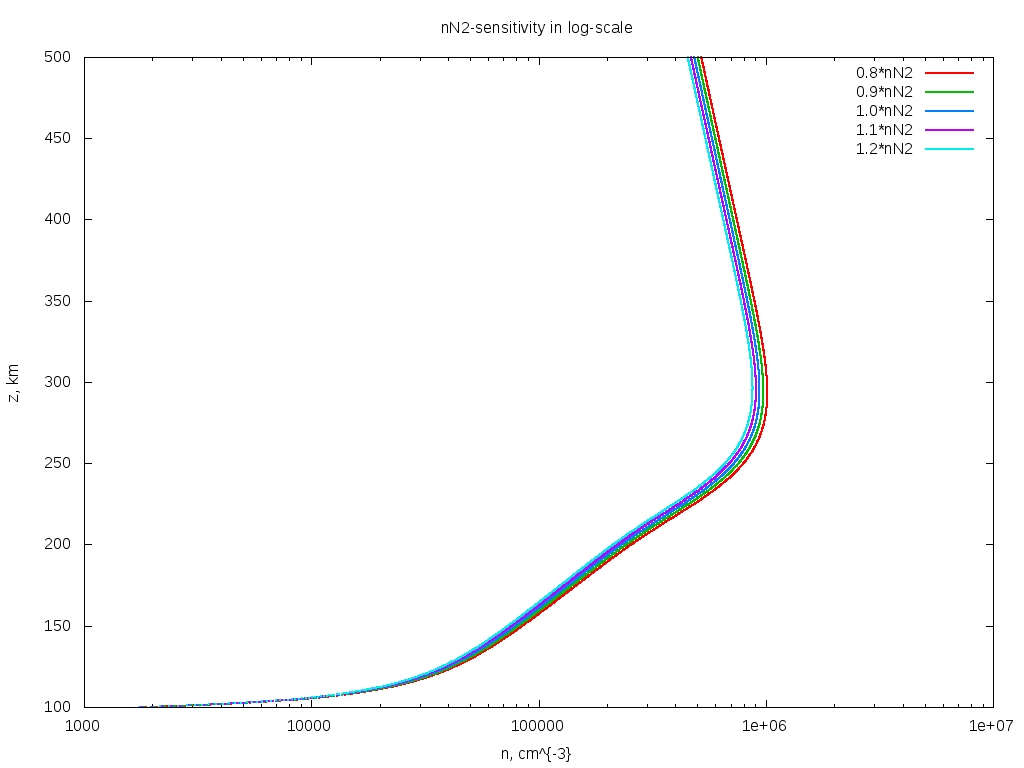
\includegraphics[scale=0.5]{nN2-sensitivity_log}}
\caption{Чувствительность к изменению концентрации азота.}
\end{figure}

\newpage

\subsection*{Суточный ход}
\subsectionmark{Суточный ход}

Полученное в предыдущем разделе стационарное решение отвечает по существу состоянию системы в один определённый момент времени, а вертикальный профиль соответствует фиксированным широте и долготе. Для моделирования суточного изменения вертикального профиля добавим зависимость от времени в слагаемое $P$, отвечающее фотоионизации.

Используем формулу $$P(z, t) =\begin{cases}
P_0(z)e^{\tau_0(z)(1-\sec\chi)}, |\chi|\leq\dfrac{\pi}{2}\\
0, |\chi|\geq\dfrac{\pi}{2}
\end{cases}$$

Здесь использованы следующие обозначения: $P_0(z)$~---~фотоионизация, использованная в одномерной модели, $\chi$~---~зенитный угол Солнца (угол между направлением на Солнце и нормалью к земной поверхности), $\tau_0(z)$~---~оптическая толщина, для вычисления которой используется формула $$\tau_0(z)=\sum_{i = N_2, O_2, O} \sigma_i^{abs}\left[\dfrac{R_0T_n}{M_i g}n_i(z)\right]= \dfrac{R_0T_n}{g}\left(\sigma_{N_2}^{abs}\dfrac{n_{N_2}(z)}{M_{N_2}}+\sigma_{O_2}^{abs}\dfrac{n_{O_2}(z)}{M_{O_2}}+\sigma_{O}^{abs}\dfrac{n_{O}(z)}{M_{O}}\right).$$

Константы $\sigma_i^{abs}$ для трёх типов нейтральных молекул известны и равны соответственно $\sigma_{N_2}^{abs}=1{,}5\cdot 10^{-17}$~см$^2$, $\sigma_{O_2}^{abs}=2\cdot 10^{-17}$~см$^2$, $\sigma_{O}^{abs}=1\cdot 10^{-17}$~см$^2$.

Характерные величины оптической толщины на различных высотах представлены в следующей таблице:

\smallskip

$$\begin{tabular}{|c|c|c|c|}
\hline
&$z_1=100$~км&$z_2=300$~км&$z_3=500$~км\\
\hline
$\tau_0$&$4\cdot 10^2$&$3\cdot 10^{-1}$&$2\cdot 10^{-4}$\\
\hline
\end{tabular}$$

\medskip

[Здесь необходимо добавить комментарии по поводу физического смысла формулы для $\tau_0$]

В предложенной формуле для фотоионизации время в качестве параметра входит лишь в зенитный угол. Кусочное задание функции $P(z, t)$ связано с приближением отсутствия фотоионизации в ночное время (Солнце не заходит за горизонт лишь при зенитных углах, не превосходящих $90^\circ$.

Зависимость зенитного угла от времени даётся следующими формулами: $$\cos\chi = \sin\varphi\cdot\sin\delta-\cos\varphi\cdot\cos\delta\cdot\cos\omega t$$

Здесь $\omega$~---~угловая скорость вращения Земли, $\varphi$~---~широта, а $\delta$~---~склонение Солнца, тангенс которого определяется формулой $$\tg\delta = \tg 23{,}5^\circ \cdot \sin\left(2\pi\cdot\dfrac{d-80}{365}\right),$$ где $d$~---~номер дня от начала года. 

В ходе численного эксперимента по моделированию суточного хода в одномерной модели вычисляется стационарное решение одномерной задачи при дневном значении $P(z)$, а затем итерации по времени продолжаются с уже меняющимся $P(z, t)$ в соответствии со введённой формулой.

Результаты представлены следующим графиком~---~трёхмерной поверхностью, построенной над плоскостью $(z, t)$:

\begin{figure}[H]
\center{
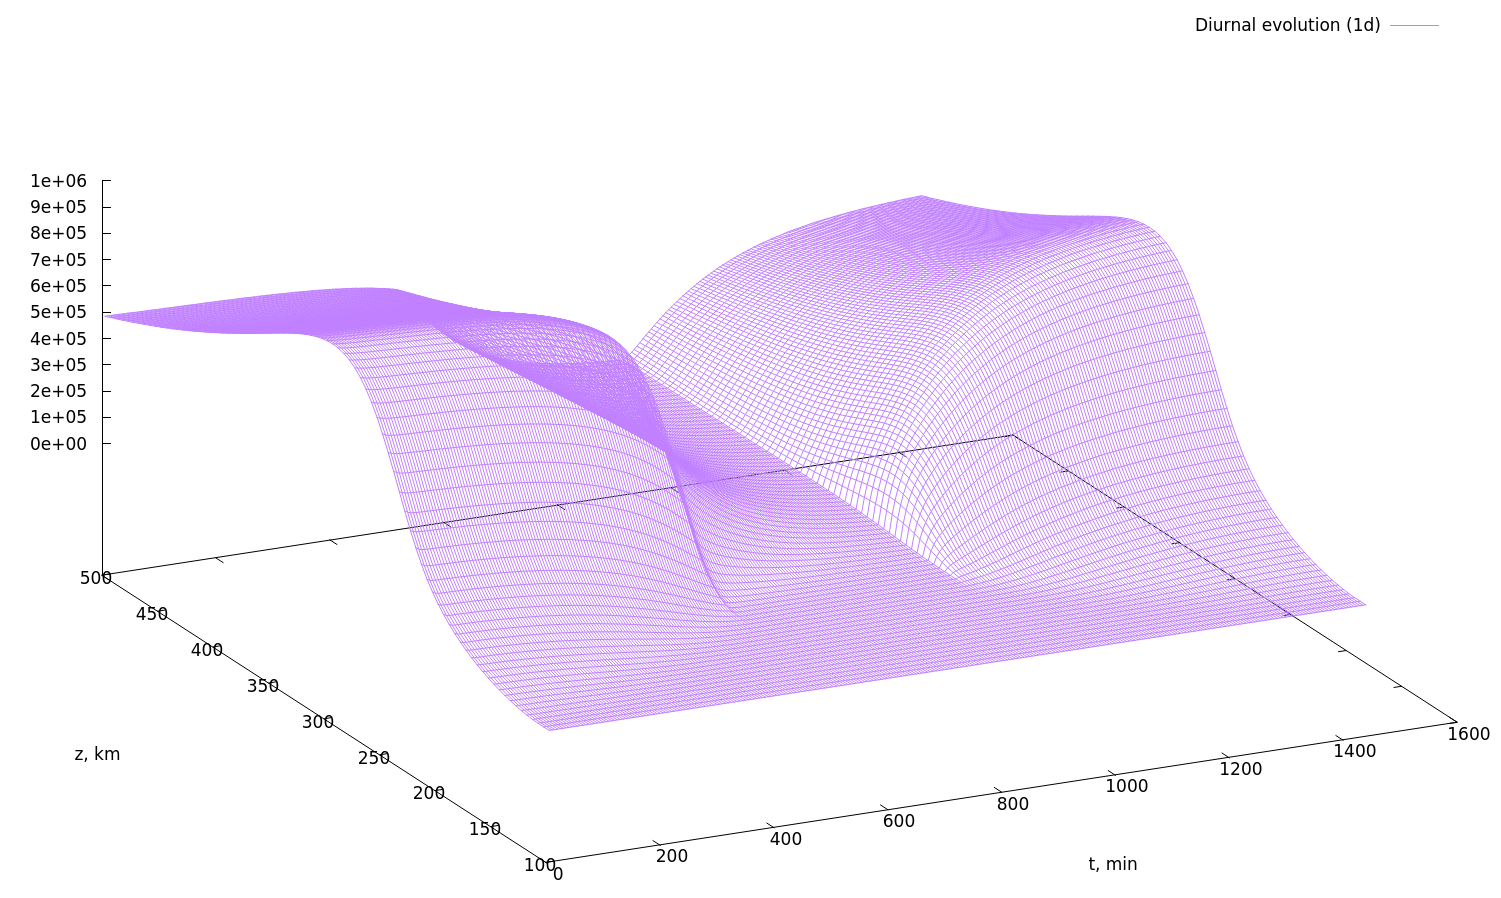
\includegraphics[scale=0.3]{diurnal_1d}}
\caption{Суточный ход в одномерной модели с добавлением зависимости фотоионизации от зенитного угла.}
\end{figure}

Видно, что за сутки решение восстанавливается. Кроме того, после зануления $P$ при зенитных углах больше $90^\circ$ начинается спад электронной концентрации, сопровождающийся изломом по времени (в соответствующий  момент $P$, входящее в уравнение, также терпит излом).

Отметим также, что при обнулении $P$ решение (начиная со стационарного) падает почти до нуля приблизительно за $6$ часов.

\bigskip

\newpage 

\subsection*{Учёт проекции на магнитную силовую линию}
\subsectionmark{Учёт проекции на магнитную силовую линию}

Учтём теперь широтную зависимость в уравнении. Простейший способ~---~замена коэффициента диффузии $D$ на $D\sin^2I$, где $I$~---~угол наклонения магнитных силовых линий, $I \approx \arctg(2\tg \varphi)$, $\varphi$~---~широта ($\varphi \in [-90^\circ; +90^\circ]$). При этом уравнение заменится на следующее:
$$\dfrac{\partial n}{\partial t} =P-kn+\dfrac{\partial}{\partial z}\left[\sin^2I\left(D\dfrac{\partial n}{\partial z} + \left(\dfrac{1}{T_p}\dfrac{\partial T_p}{\partial z}+\dfrac{1}{H}\right) n\right)\right]$$

В рассматриваемой постановке широта $\varphi$~---~внешний задаваемый параметр. При фиксированном $\varphi$ уравнение, как и раньше, имеет стационарное решение.

Особенность данной постановки состоит в том, что на экваторе при $\varphi=0$ уравнение вырождается: ненулевыми остаются только производная по времени в левой части и $P-kn$ в правой. Этот эффект не соответствует никакому физическому явлению

Результаты расчётов суточного хода при $\varphi = -70^\circ, -40^\circ, -10^\circ$ приведены на следующих графиках:

\begin{figure}[H]
\center{
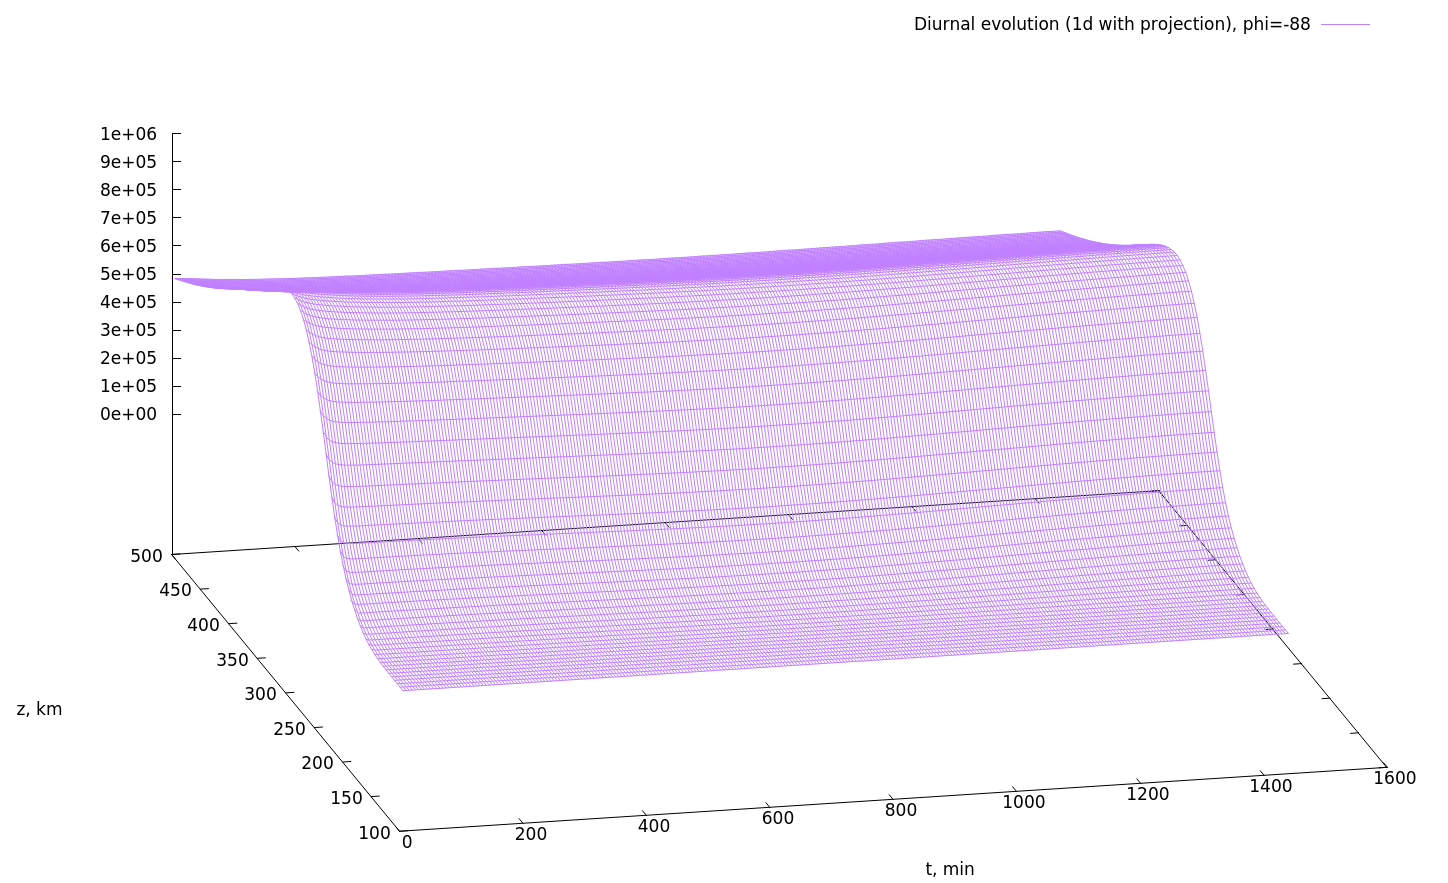
\includegraphics[scale=0.3]{diurnal_projection_-88}}
\caption{Суточный ход в одномерной модели с учётом проекции на магнитную силовую линию, $\varphi = -88^\circ$.}
\end{figure}

\begin{figure}[H]
\center{
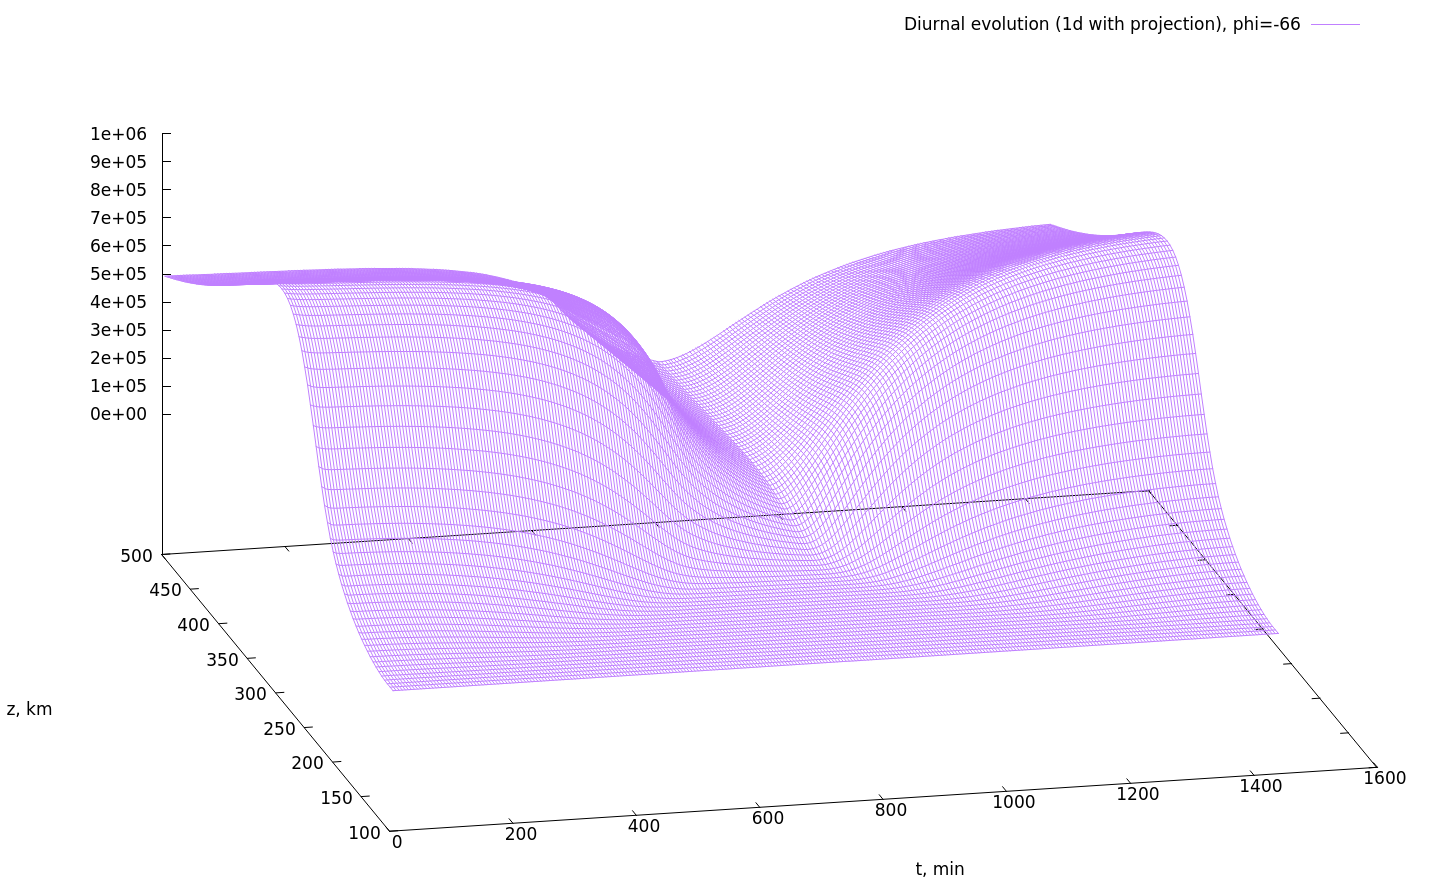
\includegraphics[scale=0.3]{diurnal_projection_-66}}
\caption{Суточный ход в одномерной модели с учётом проекции на магнитную силовую линию, $\varphi = -66^\circ$.}
\end{figure}

\begin{figure}[H]
\center{
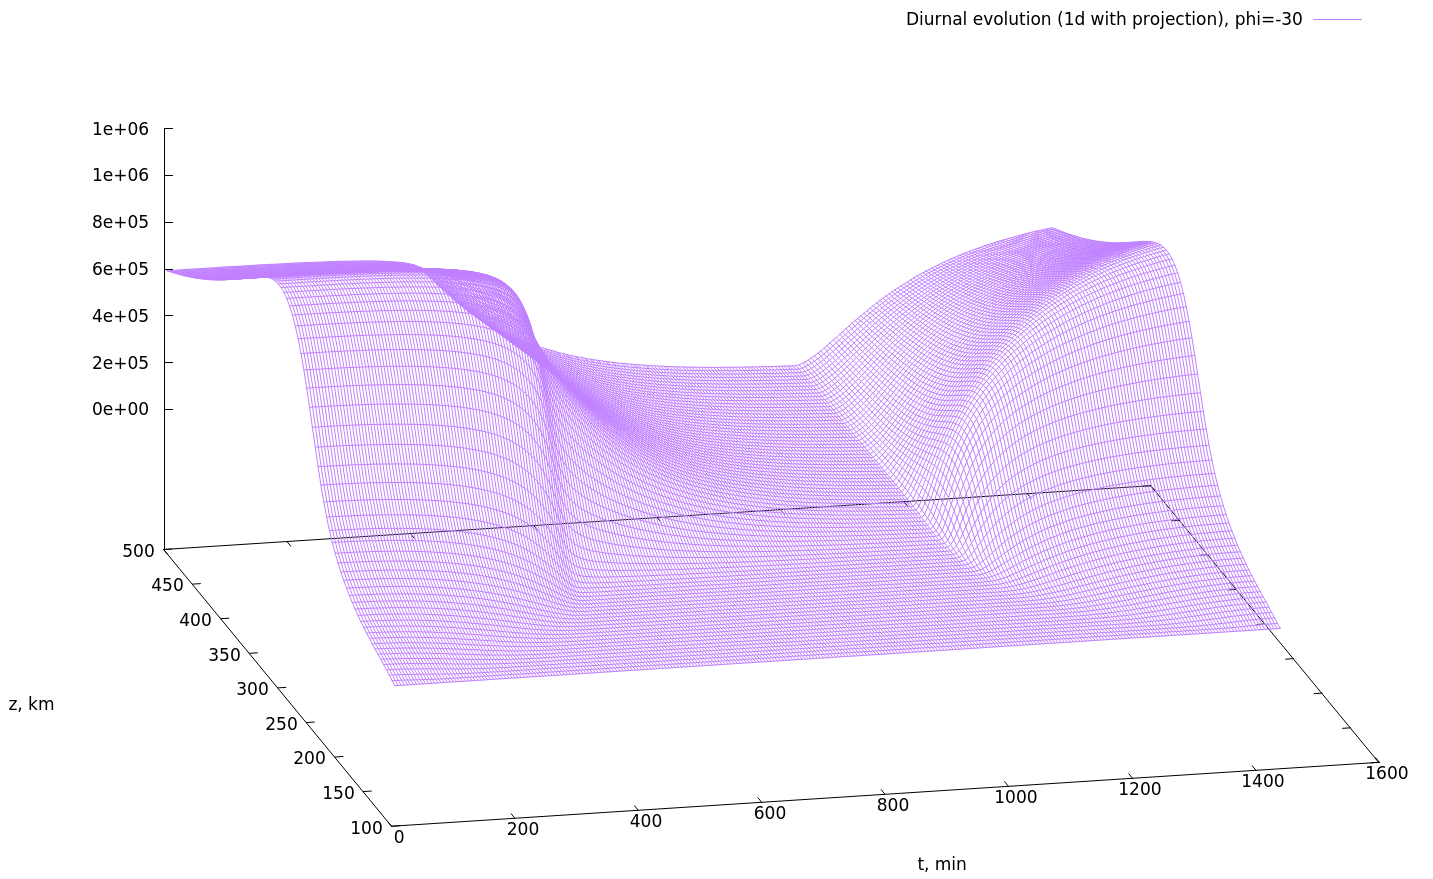
\includegraphics[scale=0.3]{diurnal_projection_-30}}
\caption{Суточный ход в одномерной модели с учётом проекции на магнитную силовую линию, $\varphi = -30^\circ$.}
\end{figure}

\begin{figure}[H]
\center{
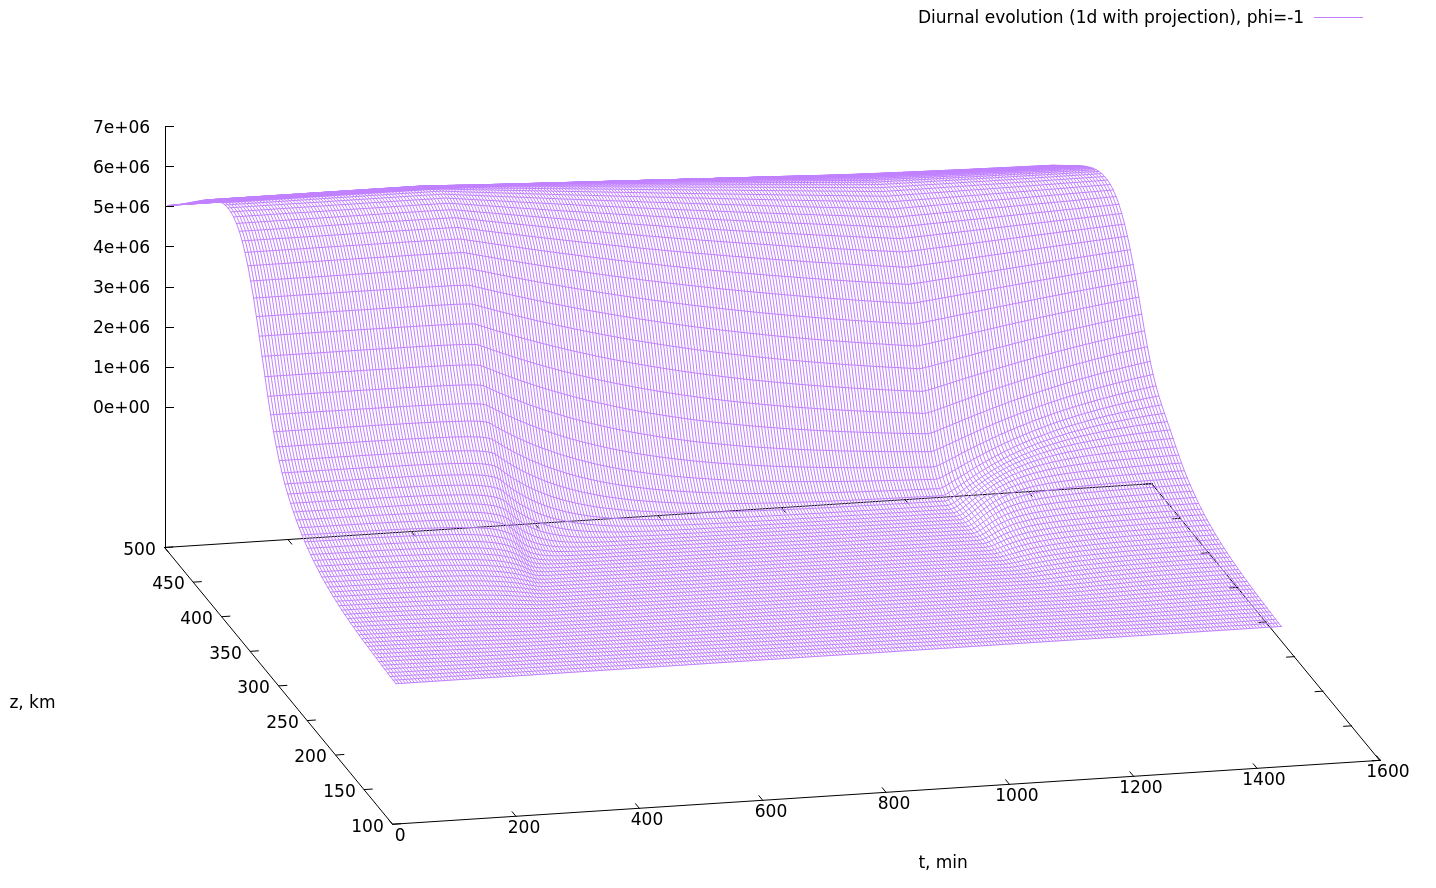
\includegraphics[scale=0.3]{diurnal_projection_-2}}
\caption{Суточный ход в одномерной модели с учётом проекции на магнитную силовую линию, $\varphi = -2^\circ$.}
\end{figure}

\newpage 

\subsection*{Квазидвумерная постановка}
\subsectionmark{Квазидвумерная постановка}

Более точный учёт широтной зависимости решения приводит к двумерной задаче:

$$\dfrac{\partial n}{\partial t} =P-kn+\dfrac{\partial}{\partial z}\biggl[D\sin^2 I\left(\dfrac{\partial n}{\partial z}+\left(\dfrac{1}{T_p}\dfrac{\partial T_p}{\partial z}+\dfrac{1}{H}\right)n\right)-$$ $$-\dfrac{1}{a}D\sin I\cos I\left(\dfrac{\partial n}{\partial\varphi}+\dfrac{1}{T_p}\dfrac{\partial T_p}{\partial\varphi}n\right)\biggr]$$

Заменим $u = \dfrac{1}{T_p}\dfrac{\partial T_p}{\partial z}+\dfrac{1}{H}$. Для использования уже имеющегося программного кода в применении уже к данной двумерной задаче используем следующую разностную схему: для смешанной производной $\dfrac{\partial}{\partial z}\dfrac{\partial n}{\partial \varphi}$ запишем $$\dfrac{\partial}{\partial z}\dfrac{\partial n}{\partial \varphi}=\dfrac{\partial}{\partial z}\left(n\dfrac{1}{n}\dfrac{\partial n}{\partial \varphi}\right) = \dfrac{\partial}{\partial z}\left(n\dfrac{\partial \ln n}{\partial \varphi}\right)$$

Введём обозначение $u_\varphi=-\dfrac{1}{a}D\sin I \cos I\dfrac{\partial \ln n}{\partial \varphi}=-\dfrac{1}{a}D\sin I \cos I\dfrac{1}{n}\dfrac{\partial n}{\partial \varphi}.$ Для рассматриваемого уравнения $u_\varphi$~---~это добавка к эффективной скорости, связанная со смешанной производной по $\varphi$.

Используем для численного решения нелинейную схему: будем вычислять решение, последовательно перемещаясь по временным слоям, причем $u_\varphi$ будем брать на основании данных с предыдущего временного слоя, а $n$~---~со следующего.

Для рассматриваемого уравнения в результате применяется та же разностная схема с центральными разностями, что и для одномерного уравнения, но возникает добавка, связанная с последним слагаемым. Для этого слагаемого использованы две различные разностные аппроксимации:
\begin{itemize}
\item[•] Схема направленных разностей с учётом возможной знакопеременности эффективной скорости: $\dfrac{|u_\varphi|+u_\varphi}{2}\cdot\dfrac{n_{i+1}-n_i}{h_i} + \dfrac{|u_\varphi|-u_\varphi}{2}\cdot\dfrac{n_{i-1}-n_i}{h_{i-1}}$
\item[•] Схема центральных разностей: $\dfrac{(u_\varphi)_{i+1}n_{i+1}-(u_\varphi)_{i-1}n_{i-1}}{h_{i-1}+h_{i+1}}$
\end{itemize}
В обоих случаях концентрации $n$ берутся со следующего временного слоя~---~схема неявная.

\smallskip

При этом сама эффективная скорость может быть вычислена двумя способами: 
\begin{itemize}
\item[•] Первый способ~---~применение формулы центральной разности к производной по $\varphi$ для логарифма в формуле $u_\varphi$ $$u_\varphi\approx \dfrac{\ln n^j_i(\varphi+\Delta\varphi)-\ln n^j_i(\varphi-\Delta\varphi}{2\Delta\varphi};$$ 
\item[•] Второй способ~---~без привлечения логарифма использовать формулу $$u\varphi \approx \dfrac{2}{n_i^j(\varphi+\Delta\varphi)+n_i^j(\varphi-\Delta\varphi)}\cdot\dfrac{n_i^j(\varphi+\Delta\varphi)-n_i^j(\varphi-\Delta\varphi)}{2\Delta\varphi}.$$
\end{itemize}

Численные эксперименты показали, что обе формулы для $u_\varphi$ дают один и тот же результат. Более того, на практике решение никогда не достигает чистого нуля, поэтому отдельные кусочные задания формул для $u_\varphi$ при нулевых значениях $n$ на предыдущем временном слое никак не отражаются на получаемом решении. Тем не менее, вторая формула более удобна для анализа асимптотического поведения $u_\varphi$ при приближении $n$ к нулю.

Для вычисления решения на следующем временном слое используются граничные условия как по $z$, так и по $\varphi$: на полюсах решение полагается тождественно равным стационарному решению одномерной задачи. Это позволяет сохранить непрерывность решения в зависимости от $\varphi \in [-90^\circ; 90^\circ]$. На нижней границе по $z$ ставится граничное условие типа Дирихле~---~решение совпадает с отношением $\dfrac{P(100\mbox{ km}, t)}{k(100\mbox{ km})}$. Верхнее граничное условие, как и ранее,~---~постоянство полного потока (с учётом добавки к эффективной скорости в виде $u_\varphi$). В разностной аппроксимации верхнего граничного условия используется центральная разность, в результате чего эта аппроксимация оказывается согласованной со схемой центральных разностей для рассматриваемого уравнения.

На следующих графиках представлен суточный ход при тех же широтах, что и в случае одномерного уравнения с $z$-проекцией. Существенное отличие наблюдается в характере решения вблизи экватора~---~уравнение не вырождается.

\begin{figure}[H]
\center{
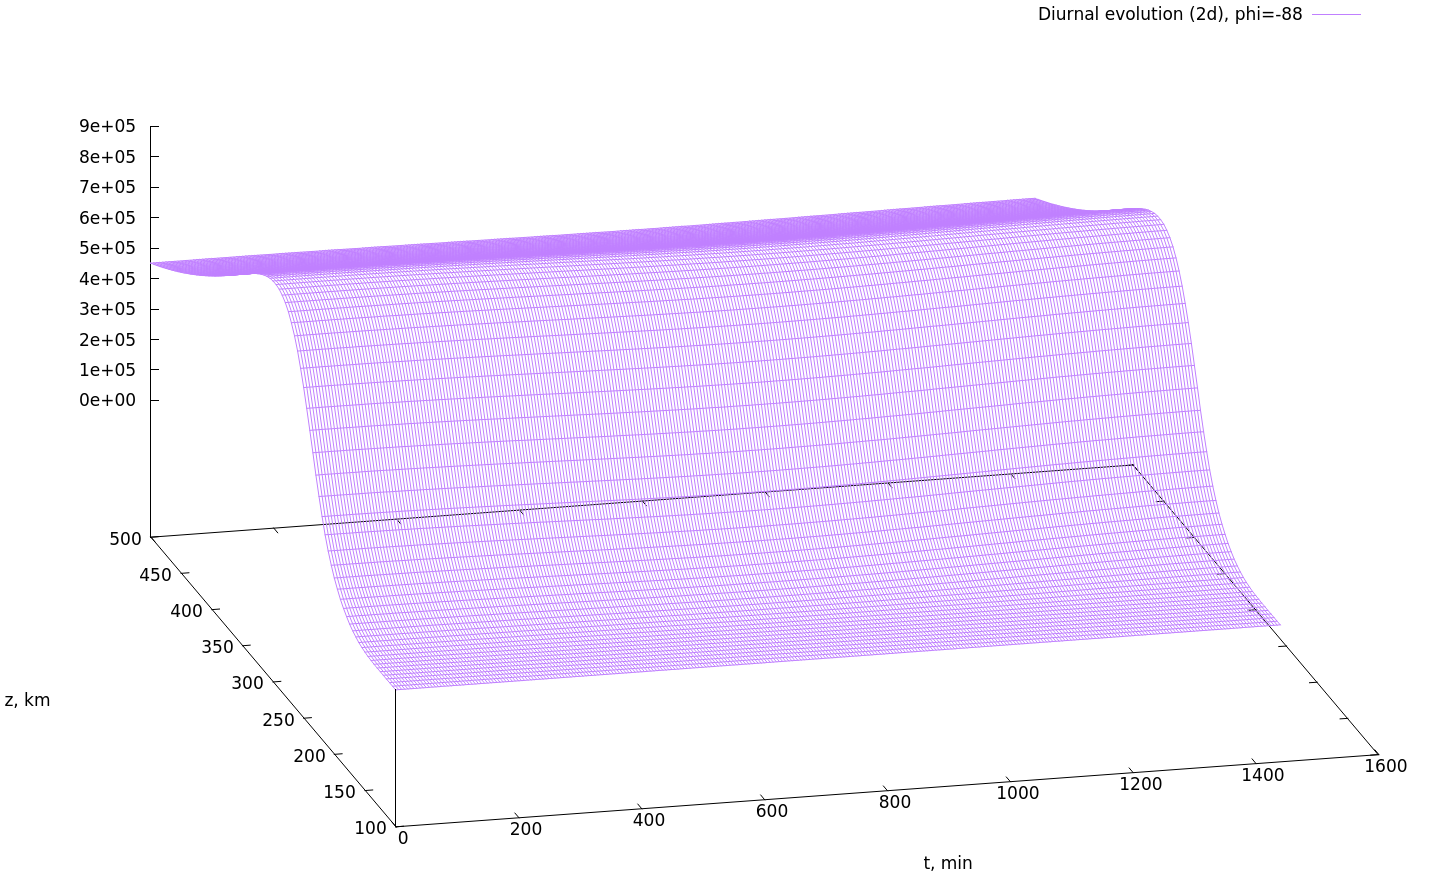
\includegraphics[scale=0.3]{diurnal_2d_-88}}
\caption{Суточный ход в квазидвумерной модели, $\varphi = -88^\circ$.}
\end{figure}

\begin{figure}[H]
\center{
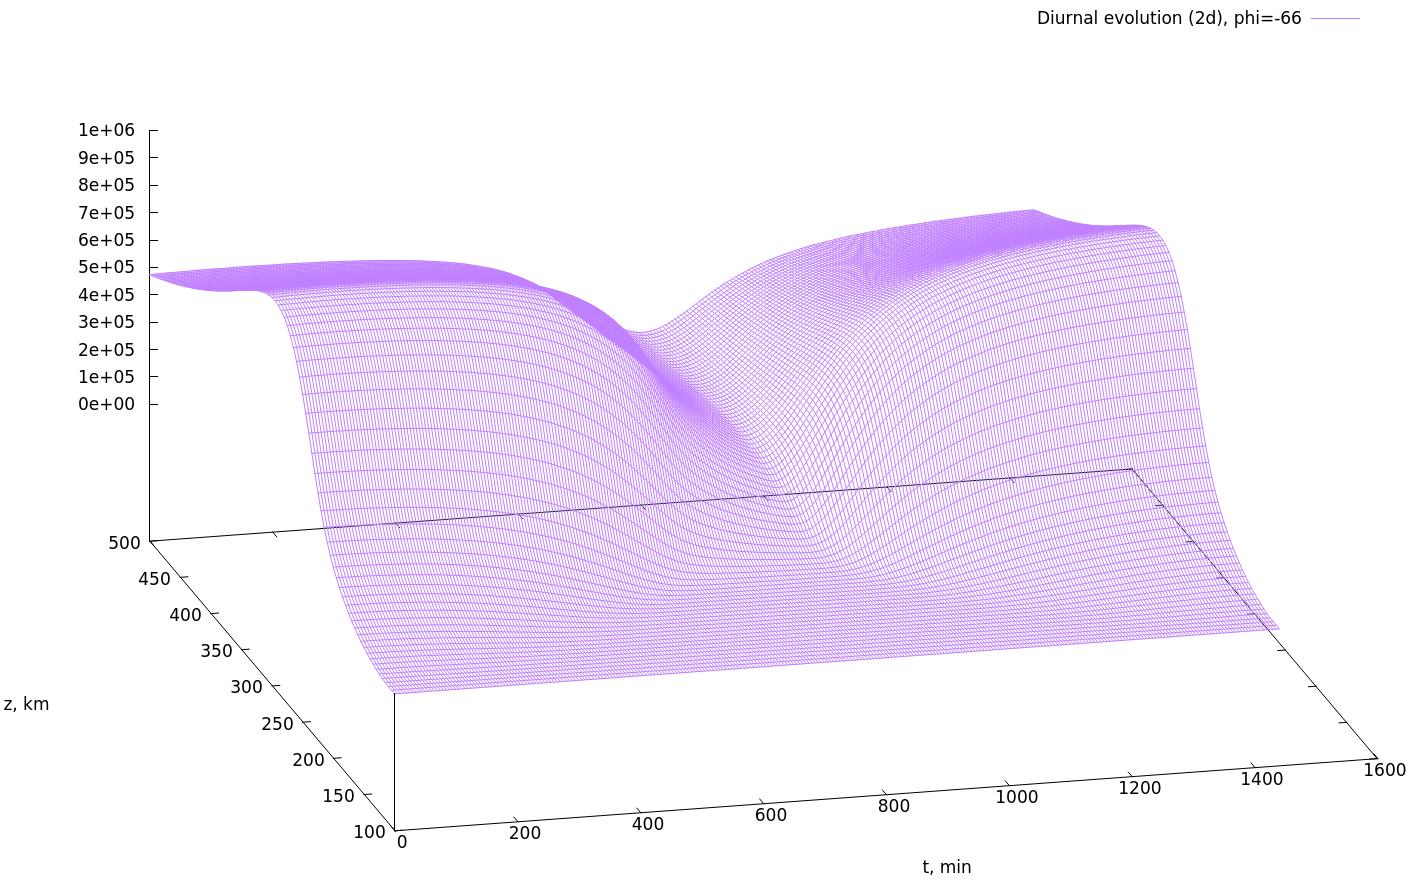
\includegraphics[scale=0.3]{diurnal_2d_-66}}
\caption{Суточный ход в квазидвумерной модели, $\varphi = -66^\circ$.}
\end{figure}

\begin{figure}[H]
\center{
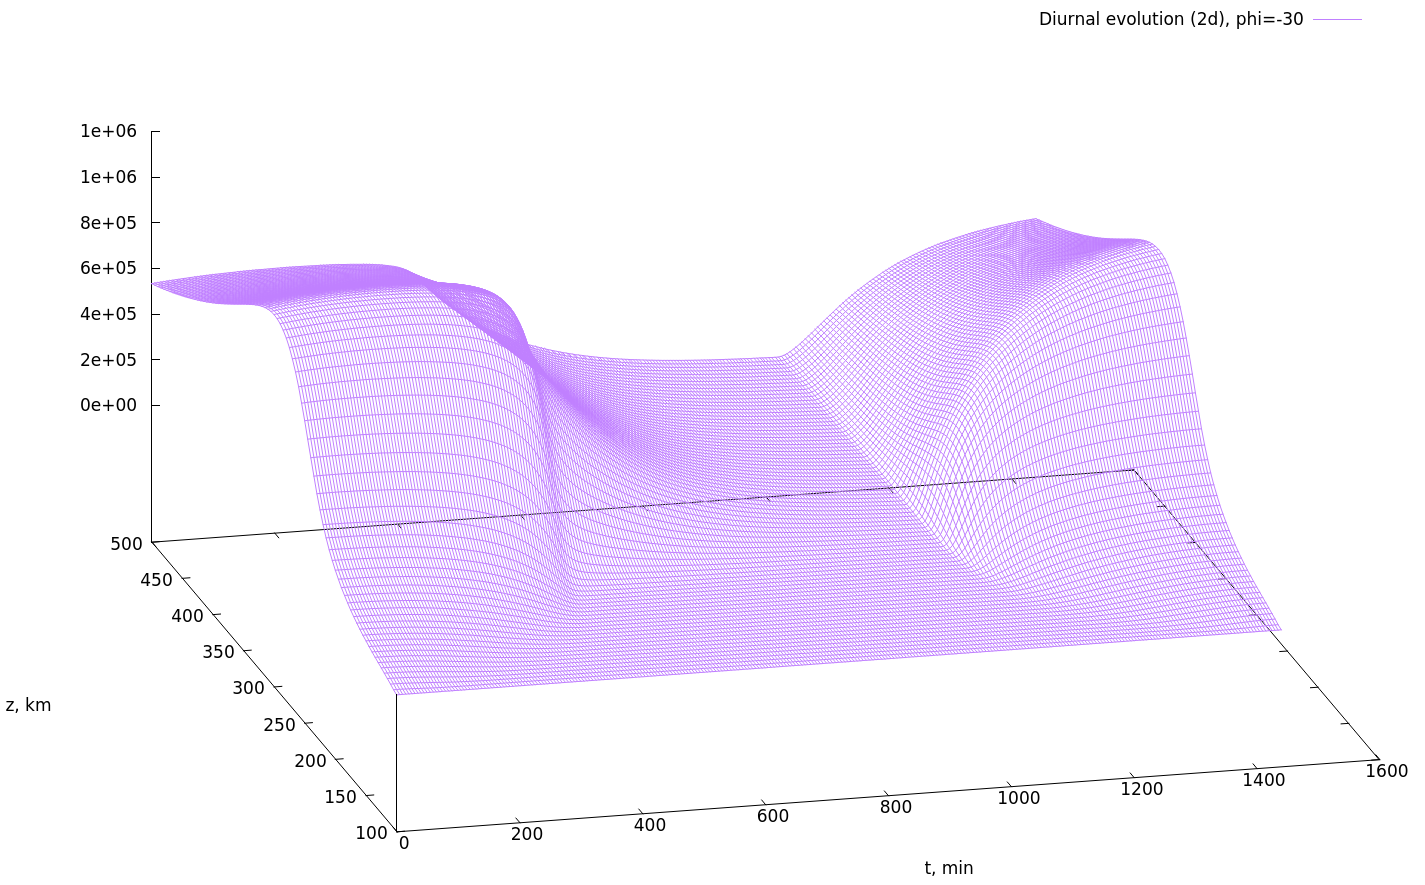
\includegraphics[scale=0.3]{diurnal_2d_-30}}
\caption{Суточный ход в квазидвумерной модели, $\varphi = -30^\circ$.}
\end{figure}

\begin{figure}[H]
\center{
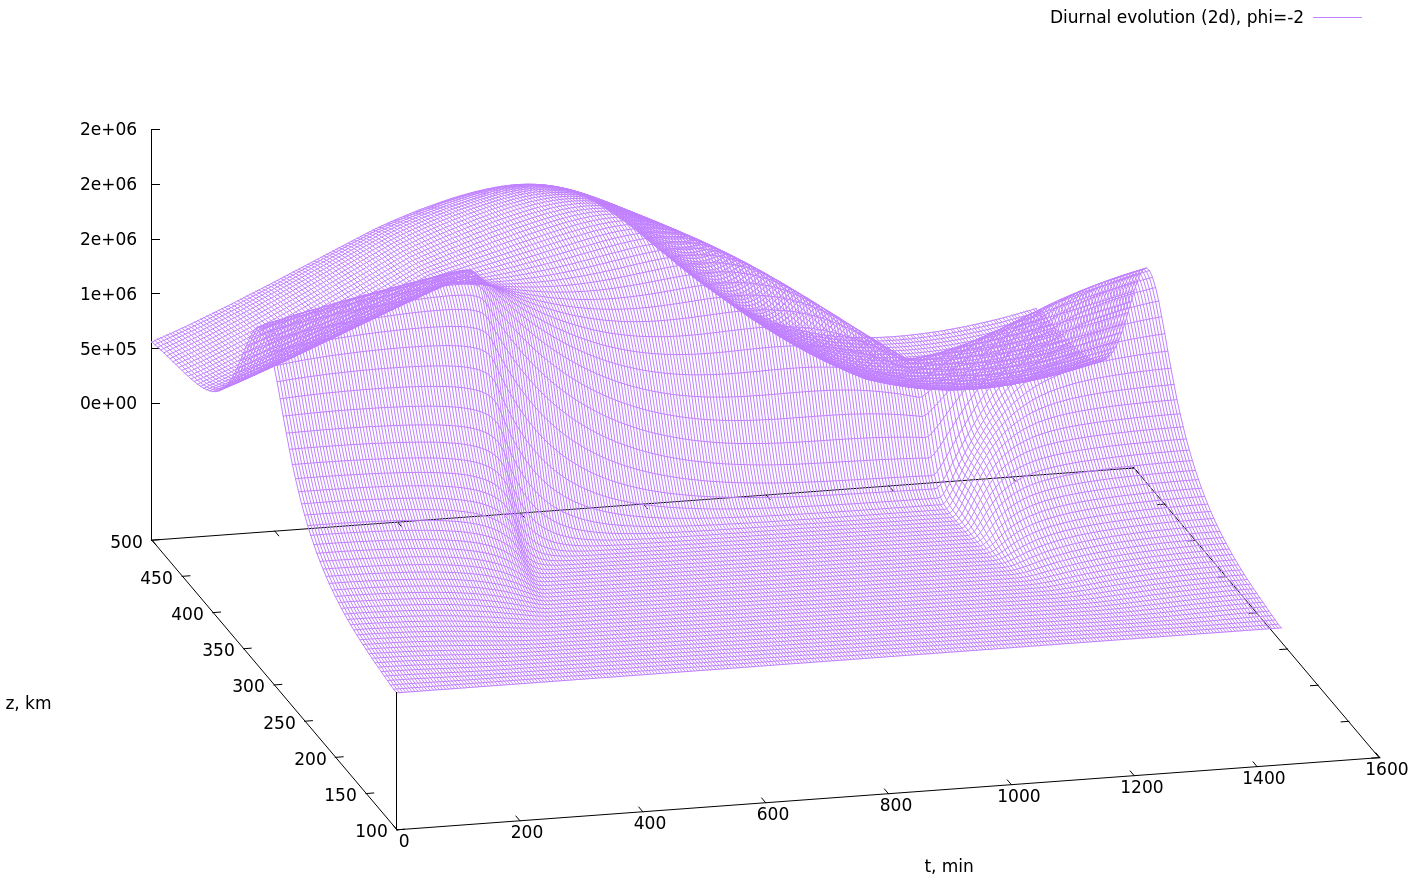
\includegraphics[scale=0.3]{diurnal_2d_-2}}
\caption{Суточный ход в одномерной модели с учётом проекции на магнитную силовую линию, $\varphi = -2^\circ$.}
\end{figure}

\subsection*{Сравнение стационарных решений в различных постановках}
\subsectionmark{Сравнение стационарных решений в различных постановках}

Различные постановки используются для учёта наклонения магнитных силовых линий. Для исследования и сравнения качественных отличий полученных результатов установим не зависящую от времени ионизацию $P(z, t) \equiv P_0(z)$ и изучим сходимости к стационарным решениям с одних и тех же начальных условий~---~вектора с компонентами, равными единице (такой вектор отвечает <<почти нулевому>> решению, при этом даёт возможность использовать схемы, применение которых к случаю нулевых значений затруднено, как, например, в случае логарифма для $u_\varphi$). 


\end{document}



